\documentclass[runningheads]{llncs}
\usepackage{booktabs}
\usepackage{multirow}
\usepackage{amsmath}
\usepackage{graphicx}
\usepackage{xcolor}

\begin{document}

\title{Tables Preview --- DP-Shampoo MICCAI 2026}
\maketitle

% =============================================================================
% MICCAI 2026 Paper Tables — DP-Shampoo
% Requires: booktabs, multirow, amsmath
% =============================================================================

% -----------------------------------------------------------------------------
% Table 1: Main Results (eps=8.0)
% -----------------------------------------------------------------------------
\begin{table}[t]
\centering
\caption{Segmentation performance (Dice score, mean $\pm$ std over 3 seeds) at
  $\varepsilon{=}8.0$, $\delta{=}10^{-5}$.
  \textbf{Bold}: best DP method per dataset.
  $\Delta$: improvement over DP-SGD in percentage points.
  Oracle uses private training data for preconditioner estimation (upper bound);
  Synthetic uses generated data only.}
\label{tab:main}
\setlength{\tabcolsep}{3.5pt}
\begin{tabular}{@{}llcccc@{}}
\toprule
\multirow{2}{*}{\textbf{Method}} &
\multirow{2}{*}{\textbf{Precond.\ Data}} &
\multicolumn{2}{c}{\textbf{Kvasir-SEG}} &
\multicolumn{2}{c}{\textbf{Oxford-IIIT Pet}} \\
\cmidrule(lr){3-4} \cmidrule(l){5-6}
& & Dice $\uparrow$ & $\Delta$ & Dice $\uparrow$ & $\Delta$ \\
\midrule
Non-private    & ---       & $.737 \pm .016$  & ---   & $.859 \pm .004$  & --- \\
\midrule
DP-SGD         & ---       & $.453 \pm .011$  & ---   & $.697 \pm .004$  & --- \\
AdaDPS         & Oracle    & $\mathbf{.513 \pm .006}$  & $\mathbf{+6.0}$  & $.661 \pm .021$  & $-$3.6 \\
AdaDPS         & Synthetic & $.510 \pm .002$  & +5.7  & $.697 \pm .006$  & +0.0 \\
DP-Shampoo     & Oracle    & $.503 \pm .004$  & +5.0  & $\mathbf{.715 \pm .009}$ & $\mathbf{+1.8}$ \\
DP-Shampoo     & Synthetic & $.509 \pm .006$  & +5.6  & $.714 \pm .006$ & +1.7 \\
\bottomrule
\end{tabular}
\end{table}


% -----------------------------------------------------------------------------
% Table 2: Epsilon Sweep — Kvasir-SEG
% -----------------------------------------------------------------------------
\begin{table}[t]
\centering
\caption{Privacy--utility tradeoff on Kvasir-SEG (Dice score, mean $\pm$ std, 3 seeds).
  \textbf{Bold}: best DP method per~$\varepsilon$.}
\label{tab:eps_kvasir}
\setlength{\tabcolsep}{3.5pt}
\begin{tabular}{@{}lcccc@{}}
\toprule
\textbf{Method} &
$\varepsilon{=}1$ & $\varepsilon{=}2$ & $\varepsilon{=}4$ & $\varepsilon{=}8$ \\
\midrule
DP-SGD                       & $.272 \pm .005$ & $.287 \pm .008$ & $.442 \pm .007$ & $.453 \pm .011$ \\
AdaDPS (synth.)      & $\mathbf{.337 \pm .028}$ & $\mathbf{.452 \pm .009}$ & $\mathbf{.495 \pm .004}$ & $\mathbf{.510 \pm .002}$ \\
Shampoo (oracle)     & $.293 \pm .025$ & $.441 \pm .016$ & $.488 \pm .004$ & $.503 \pm .004$ \\
Shampoo (synth.)     & $.282 \pm .008$ & $.443 \pm .003$ & $.490 \pm .006$ & $.509 \pm .006$ \\
\midrule
Non-private & \multicolumn{4}{c}{$.737 \pm .016$} \\
\bottomrule
\end{tabular}
\end{table}


% -----------------------------------------------------------------------------
% Table 3: Epsilon Sweep — Oxford-IIIT Pet
% -----------------------------------------------------------------------------
\begin{table}[t]
\centering
\caption{Privacy--utility tradeoff on Oxford-IIIT Pet (Dice score, mean $\pm$ std, 3 seeds).
  \textbf{Bold}: best DP method per~$\varepsilon$.}
\label{tab:eps_pet}
\setlength{\tabcolsep}{3.5pt}
\begin{tabular}{@{}lcccc@{}}
\toprule
\textbf{Method} &
$\varepsilon{=}1$ & $\varepsilon{=}2$ & $\varepsilon{=}4$ & $\varepsilon{=}8$ \\
\midrule
DP-SGD                       & $.657 \pm .006$ & $.671 \pm .009$ & $.687 \pm .004$ & $.697 \pm .004$ \\
AdaDPS (synth.)      & $.659 \pm .007$ & $.673 \pm .003$ & $.687 \pm .004$ & $.697 \pm .006$ \\
Shampoo (oracle)     & $.664 \pm .004$ & $\mathbf{.682 \pm .002}$ & $\mathbf{.704 \pm .012}$ & $\mathbf{.715 \pm .009}$ \\
Shampoo (synth.)     & $\mathbf{.667 \pm .008}$ & $.683 \pm .002$ & $.692 \pm .001$ & $.714 \pm .006$ \\
\midrule
Non-private & \multicolumn{4}{c}{$.859 \pm .004$} \\
\bottomrule
\end{tabular}
\end{table}


% -----------------------------------------------------------------------------
% Compact Alternative: Combined Epsilon Sweep (saves space)
% Use this instead of Tables 2+3 if space is tight
% -----------------------------------------------------------------------------
\begin{table}[t]
\centering
\caption{Privacy--utility tradeoff (Dice score, mean $\pm$ std, 3 seeds).
  \textbf{Bold}: best DP method per dataset and~$\varepsilon$.}
\label{tab:eps_combined}
\setlength{\tabcolsep}{3pt}
\small
\begin{tabular}{@{}llcccc@{}}
\toprule
\textbf{Dataset} & \textbf{Method} &
$\varepsilon{=}1$ & $\varepsilon{=}2$ & $\varepsilon{=}4$ & $\varepsilon{=}8$ \\
\midrule
\multirow{5}{*}{\rotatebox[origin=c]{90}{\textsc{Kvasir}}}
& DP-SGD              & $.272_{\pm.005}$ & $.287_{\pm.008}$ & $.442_{\pm.007}$ & $.453_{\pm.011}$ \\
& AdaDPS (synth.)     & $\mathbf{.337}_{\pm.028}$ & $\mathbf{.452}_{\pm.009}$ & $\mathbf{.495}_{\pm.004}$ & $\mathbf{.510}_{\pm.002}$ \\
& Shampoo (oracle)    & $.293_{\pm.025}$ & $.441_{\pm.016}$ & $.488_{\pm.004}$ & $.503_{\pm.004}$ \\
& Shampoo (synth.)    & $.282_{\pm.008}$ & $.443_{\pm.003}$ & $.490_{\pm.006}$ & $.509_{\pm.006}$ \\
& \textcolor{gray}{Non-private} & \multicolumn{4}{c}{\textcolor{gray}{$.737 \pm .016$}} \\
\midrule
\multirow{5}{*}{\rotatebox[origin=c]{90}{\textsc{Pet}}}
& DP-SGD              & $.657_{\pm.006}$ & $.671_{\pm.009}$ & $.687_{\pm.004}$ & $.697_{\pm.004}$ \\
& AdaDPS (synth.)     & $.659_{\pm.007}$ & $.673_{\pm.003}$ & $.687_{\pm.004}$ & $.697_{\pm.006}$ \\
& Shampoo (oracle)    & $.664_{\pm.004}$ & $\mathbf{.682}_{\pm.002}$ & $\mathbf{.704}_{\pm.012}$ & $\mathbf{.715}_{\pm.009}$ \\
& Shampoo (synth.)    & $\mathbf{.667}_{\pm.008}$ & $.683_{\pm.002}$ & $.692_{\pm.001}$ & $.714_{\pm.006}$ \\
& \textcolor{gray}{Non-private} & \multicolumn{4}{c}{\textcolor{gray}{$.859 \pm .004$}} \\
\bottomrule
\end{tabular}
\end{table}


\begin{figure}[t]
\centering
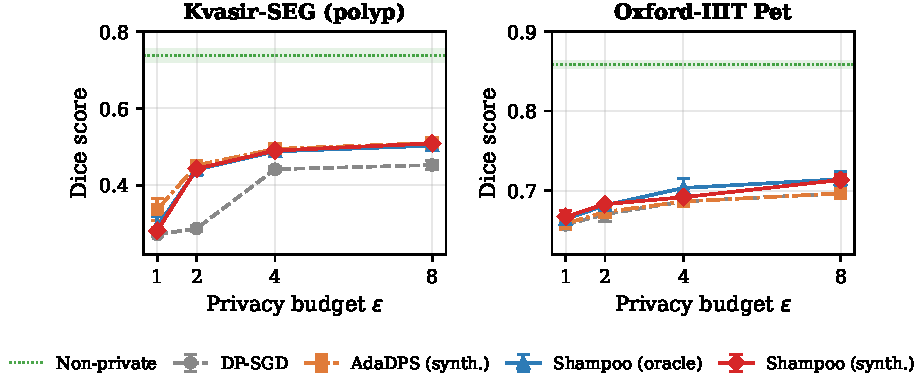
\includegraphics[width=\textwidth]{epsilon_sweep.pdf}
\caption{Privacy--utility tradeoff across $\varepsilon \in \{1,2,4,8\}$.
  DP-Shampoo with synthetic data (red) consistently matches or outperforms
  vanilla DP-SGD (gray) and is competitive with the oracle upper bound (blue).
  Green band: non-private baseline $\pm$ 1 std.}
\label{fig:eps_sweep}
\end{figure}

\begin{figure}[t]
\centering
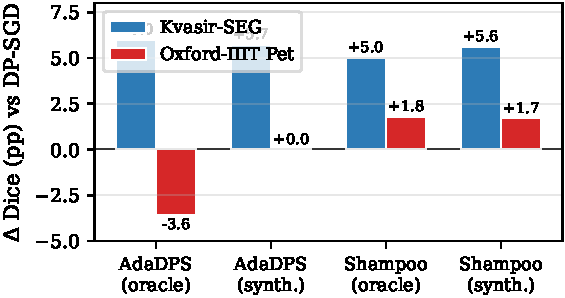
\includegraphics[width=0.65\textwidth]{improvement_bars.pdf}
\caption{Dice improvement (percentage points) over DP-SGD at $\varepsilon{=}8.0$.
  Shampoo is the only preconditioner that consistently improves across both datasets.
  AdaDPS with oracle data hurts on Pet ($-3.6$\,pp), while Shampoo with synthetic data
  achieves $+5.6$\,pp and $+1.7$\,pp on Kvasir and Pet respectively.}
\label{fig:improvement}
\end{figure}

\end{document}
